% Part VI: the new theory (section 13) and appendices
\addcontentsline{toc}{part}{Part VI \quad The new theory}
\section{Putting it together: the tilted walk and the learned pair energy}\label{sec:synthesis}

\subsection{The question, restated with everything we now have}

We observe many short sequences $x_{1:L}$, each a stationary snapshot of the $\phi^4$ field (\S\ref{sec:allencahn}),
standardised and passed through the channel \eqref{eq:channel} at some level $t$. We want the exact score
\eqref{eq:tweedie} at every level, which by Tweedie is the posterior mean, which by \S\ref{sec:bp} is one
forward--backward pass \emph{if we know the kernel $K$}. So the whole problem is to \emph{learn the local law}
from noised data (EM, \S\ref{sec:em}) and let belief propagation compose it exactly. The theory below says which
families of local laws can contain the truth, what their parameters mean, and why the simpler alternatives fail.

\subsection{The tilted-walk identity}

\begin{proposition}[the field's kernel is a tilted random walk]\label{prop:tilt}
With $g=\psi_0D$, the ground-state kernel \eqref{eq:gst} can be written
\begin{equation}\label{eq:tiltedwalk}
  K(\phi'\mid\phi)=\frac{\N(\phi';\phi,\Th h)\;g(\phi')}{Z_g(\phi)},\qquad Z_g(\phi)=\int\N(\phi';\phi,\Th h)\,g(\phi')\dd\phi'=\frac{\lambda_0\psi_0(\phi)}{c\,D(\phi)},
\end{equation}
with $c=\sqrt{2\pi\Th h}$ the Gaussian's normalising constant.
\end{proposition}
\begin{proof}
Insert \eqref{eq:transfer} into \eqref{eq:gst}: $K=D(\phi)G(\phi'-\phi)D(\phi')\psi_0(\phi')/(\lambda_0\psi_0(\phi))=G(\phi'-\phi)g(\phi')\cdot D(\phi)/(\lambda_0\psi_0(\phi))$. The
eigen-equation $\int\mathsf T(\phi,\phi')\psi_0(\phi')\dd\phi'=\lambda_0\psi_0(\phi)$ reads $D(\phi)\int G(\phi'-\phi)g(\phi')\dd\phi'=\lambda_0\psi_0(\phi)$, which is the
normaliser. Replace $G$ by $c\,\N(\cdot;\phi,\Th h)$.
\end{proof}

In words: \emph{take a Gaussian random-walk step of variance $\Th h$, then tilt the landing point by a positive weight
$g(\phi')$, and renormalise}. The weight combines the local preference $D(\phi')=e^{-hV(\phi')/2\Th}$ with the future factor
$\psi_0(\phi')$. The normaliser $Z_g$ is the ground-state transform itself, so a model that parametrises $\log g$ and
normalises each column numerically contains the truth \emph{without ever computing $\psi_0$ or $\lambda_0$}. In
standardised units $a=\phi/s$ the step variance is $\gamma=\Th h/s^2$.

\subsection{Where the two laboratories meet, and where they part}

\begin{proposition}\label{prop:embed}
The Gaussian AR(1) kernel $\N(a';\rho a,q)$ with $0<\rho<1$ is a tilted walk, with $\gamma=q/\rho$ and the quadratic tilt
$\log g(a')=-(1-\rho)a'^2/2q$. No other AR(1) kernel $k(a'-\rho a)$ is a tilted walk.
\end{proposition}
\begin{proof}
For the first claim, complete the square: $\N(a';a,\gamma)e^{-ca'^2}$ is a Gaussian in $a'$ with mean $a/(1+2c\gamma)$ and
variance $\gamma/(1+2c\gamma)$; setting these to $\rho a$ and $q$ gives $\gamma=q/\rho$ and $2c=(1-\rho)/q$. For the second, note
that for any tilted walk the mixed derivative $\partial_a\partial_{a'}\log K=1/\gamma$ is a constant: $\log g$ depends only on
$a'$, $\log Z_g$ only on $a$, and the Gaussian contributes $aa'/\gamma$. For $k(a'-\rho a)$ the mixed derivative is
$-\rho(\log k)''(a'-\rho a)$, constant only if $\log k$ is quadratic, i.e.\ $k$ Gaussian.
\end{proof}

So the first laboratory (AR(1) chains with non-Gaussian innovations) and the second (gradient fields like
$\phi^4$) share exactly one member, the Gaussian chain. What separates them is the \emph{drift}:

\begin{proposition}[the drift is the gradient of the log-normaliser]
For a tilted walk, $\E[a'-a\mid a]=\gamma\,(\log Z_g)'(a)$.
\end{proposition}
\begin{proof}
$Z_g'(a)=\int\partial_a\N(a';a,\gamma)\,g(a')\dd a'=\int\frac{a'-a}{\gamma}\N(a';a,\gamma)g(a')\dd a'=Z_g(a)\,\E[a'-a\mid a]/\gamma$.
\end{proof}
For the field, $\log Z_g=\log\psi_0+hV/2\Th+\text{const}$ (physical units), so the expected step is
$\Th h(\log\psi_0)'(\phi)+\tfrac{h^2}{2}V'(\phi)$: a \emph{nonlinear} function that pushes the field back towards the wells.
In the limit of small $h$ the spatial profile obeys $\dd\phi=\Th(\log\psi_0)'(\phi)\dd x+\sqrt\Th\,\dd B$: the drift in space is the
log-derivative of the ground state, not $-V'$. An AR(1) kernel with any innovation law, including the paper's
mixture of Gaussians, has a \emph{linear} drift $\rho a$. It is misspecified on the field through its drift, not
through the shape of its noise, and no amount of data repairs that (\S\ref{sec:em}).

\subsection{Every tilted walk is reversible}

\begin{proposition}[reversibility and the site energy]\label{prop:rev}
For any $\gamma>0$ and positive $g$ with finite $Z_g$, the tilted walk $K_g(a'\mid a)=\N(a';a,\gamma)g(a')/Z_g(a)$ is
reversible with invariant density $\pi_g\propto g\,Z_g$. Equivalently, it is the Gibbs chain of the symmetric pair energy
\begin{equation}\label{eq:pairenergy}
  W(a,a')=\frac{(a'-a)^2}{2\gamma}+f(a)+f(a'),\qquad f=-\tfrac12\log\big(g/Z_g\big),
\end{equation}
and conversely every pair energy of this form is a tilted walk. For the $\phi^4$ field, $f(a)=\tfrac{h}{2\Th}V(sa)+\text{const}$.
\end{proposition}
\begin{proof}
$\pi_g(a)K_g(a'\mid a)\propto g(a)Z_g(a)\N(a';a,\gamma)g(a')/Z_g(a)=g(a)g(a')\N(a';a,\gamma)$, which is symmetric in $(a,a')$: detailed
balance \eqref{eq:detbal}, hence invariance. For the second form, take $u=\sqrt{g/Z_g}=e^{-f}$ and the symmetric operator
$\mathsf T_g(a,a')=u(a)\N(a';a,\gamma)u(a')$. Then $\psi=\sqrt{gZ_g}$ satisfies $\mathsf T_g\psi=u\int\N g=uZ_g=\psi$ (using $u\psi=g$), so $\psi$ is
its Perron eigenfunction with eigenvalue $1$, and its ground-state transform is
$\mathsf T_g(a,a')\psi(a')/\psi(a)=\N(a';a,\gamma)g(a')/Z_g(a)=K_g$. The converse is Proposition~\ref{prop:tilt} with $D=e^{-f}$. For the
field, $g/Z_g=c\,D^2/\lambda_0$ by \eqref{eq:tiltedwalk}, so $f=-\log D+\text{const}=hV/2\Th+\text{const}$.
\end{proof}

\begin{keyidea}
A learned transition kernel of this form and a learned symmetric pair energy are \emph{one model}. Nothing
irreversible can be learned by mistake, and a fitted kernel \emph{reads as physics}: since $\gamma=\Th h/s^2$ and
$f(a)=\tfrac{h}{2\Th}V(sa)+\text{const}$,
\begin{equation}\label{eq:readout}
  \hat\Th=\hat\gamma\,s^2/h,\qquad\hat V(\phi)=\frac{2\hat\Th}{h}\,\hat f(\phi/s)+\text{const}.
\end{equation}
The temperature is read from the bond variance alone, the potential (its barrier, its wells) from the site
energy. Numerically, on the $401$-point grid: $\pi_g$ by formula and by eigensolve agree to $4\times10^{-12}$,
detailed balance holds to $10^{-14}$, and the field's own site energy equals $\tfrac h{2\Th}V$ to $2\times10^{-10}$.
\end{keyidea}

\subsection{Three ways to learn the local law}

\begin{enumerate}
\item \textbf{The innovation mixture} (the paper's estimator): $K(a'\mid a)=\sum_cw_c\N(a';\rho a+\mu_c,s_c^2)$, $25$ parameters at
  $8$ components. Exact on the AR(1) laboratory, misspecified on the field (linear drift).
\item \textbf{A tilt basis}: $\log g=\sum_m\theta_mB_m$ with Legendre polynomials ($7$ parameters) or cubic B-splines ($25$),
  plus $\log\gamma$. For each source value the kernel is an exponential family in $\theta$, so the M-step is concave and its
  gradient is \eqref{eq:expfamgrad}: posterior transition statistics minus the kernel's own conditional expectations,
  which is Boltzmann learning without a partition function.
\item \textbf{The site energy itself} (the physicist's parametrisation): $f$ a quartic, five parameters with $\log\gamma$,
  exactly specified for $\phi^4$ because $\log g=\log\psi_f-f$ is complicated but $f$ is not. The kernel needs one
  eigensolve of the $N_g\times N_g$ operator $\mathsf T_f$ per evaluation, and the M-step's gradient needs the derivative of the
  Perron eigenvector. Differentiating $\mathsf T\psi_0=\lambda_0\psi_0$ and projecting on $\psi_n$ ($n\ge1$) gives
  $\langle\psi_n,\dd\mathsf T\psi_0\rangle+\lambda_n\langle\psi_n,\dd\psi_0\rangle=\lambda_0\langle\psi_n,\dd\psi_0\rangle$, so
  \[
    \dd\psi_0=\sum_{n\ge1}\psi_n\,\frac{\langle\psi_n,\dd\mathsf T\,\psi_0\rangle}{\lambda_0-\lambda_n},
  \]
  (the component along $\psi_0$ vanishes because $\psi_0$ stays normalised). The denominators are positive by
  Perron--Frobenius. This objective is not concave, so a step is accepted only if $Q$ increases.
\end{enumerate}

\begin{caution}
``Exactly specified up to the basis'' does not mean every fit is usable. The expected transition counts $\Xi$
vanish beyond the data's range ($|a|\gtrsim3.5$), so the likelihood says nothing about $\log g$ there. A global basis
(Legendre) can raise the tilt in that empty region and create a pocket; the kernel's own invariant law, which the
estimator uses for the first site, then sits in the pocket, and every posterior is dragged outside the data. In
the previews this happened in five of eighteen Legendre fits (risks $0.18$ to $1.79$) and in none of fifty spline
or site-energy fits. The check is the invariant law's mass beyond the data range (N-33). The site energy is
immune because $g=\psi_fe^{-f}$ decays by construction.
\end{caution}

\begin{figure}[h]\centering
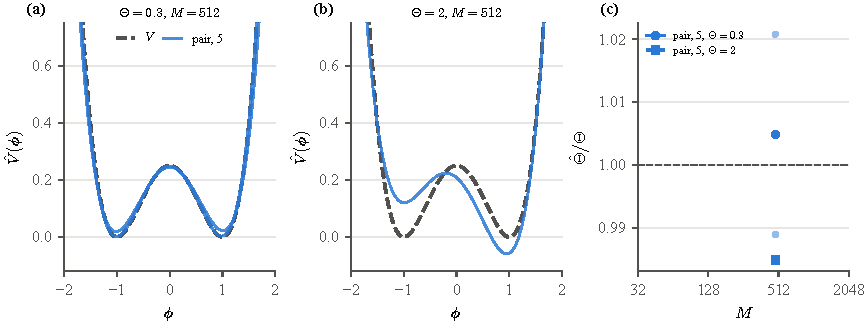
\includegraphics{fig-field-potential.pdf}
\caption{The physics read from kernels learned \emph{through the noise} (laptop preview, two seeds, not yet the
confirmatory run). (a) $\hat V$ from the five-parameter site energy at $\Th=0.3$, $M=512$ sequences, against the true
double well (dashed); a clean-data fit dotted. (b) The same at $\Th=2$, where the barrier is far below the
thermal energy and the data barely constrain it. (c) $\hat\Th/\Th$ against the number of sequences.}
\label{fig:potential}
\end{figure}

\subsection{What has been measured so far}

Table~\ref{tab:results} collects the numbers that matter for the paper, with their status. ``Frozen'' means the
output files are checksummed in the registry; ``preview'' means a laptop run on two cells and at most two seeds,
under the registered code but not the registered design. The confirmatory runs of E33 (sixteen seeds, six cells,
five kernel arms, two network architectures) are queued on the cluster.

\begin{table}[h]\centering\small
\caption{The main measurements on the $\phi^4$ laboratory. Score errors are pooled relative errors (\S\ref{sec:noise});
the base cell is $\Th=0.3$, $h=1$, $L=32$.}
\label{tab:results}
\begin{tabular}{@{}p{6.6cm}p{5.4cm}p{3.3cm}@{}}
\toprule
quantity & value & source, status \\
\midrule
Gaussian closure (linear floor), base cell & $0.269$ & E33 oracles, 16 seeds \\
floor along matched correlation, $\Th=0.3,0.5,1,2$ & $0.269,\ 0.114,\ 0.059,\ 0.041$ & E33 oracles \\
floor at fixed spacing $h=1$, $\Th=0.2\to2$ & $0.296\to0.184$, monotone & E32, frozen \\
Theorem~2 gap ratio at $t=3$ & $0.73$--$0.94$ & E32, frozen \\
mixture kernel through noise, base, $M=128$ and $512$ & $0.276,\ 0.272$ (no improvement with data) & preview \\
spline tilt through noise, base, $M=128$ and $512$ & $0.034,\ 0.039$ & preview \\
site energy through noise, base, $M=128$ and $512$ & $0.035,\ 0.021$ & preview \\
temperature read through noise, base, $M=512$ & $\hat\Th/\Th=1.005\pm0.023$, barrier $0.234$ & preview \\
clean fits, base, $M=2048$: site energy, spline, mixture & $0.005,\ 0.006,\ 0.27$ & preview \\
samples from the learned site energy: kinks, domain length & within $5\,\%$ and $2\,\%$ of the truth & preview \\
coarse kinks across lattice spacings, across strides & within $11\,\%$, within $8\,\%$ & E34, E36 \\
\bottomrule
\end{tabular}
\end{table}

Read the table as one story. The linear floor (Kalman on the covariance twin, \S\ref{sec:kalman}) leaves a quarter
of the score unexplained on the base cell, because the field's structure is non-Gaussian and the Hermite
argument (\S\ref{sec:hermite}) says that structure lives in high orders. The paper's mixture kernel cannot reach it
however much data it sees, because its drift is linear (\S\ref{sec:synthesis}). Kernels of the right class reach
errors seven to thirteen times smaller from a few hundred noised sequences, and their parameters return the temperature and
the potential that generated the data.

\subsection{Open questions}

\begin{itemize}
\item Do the confirmatory runs (sixteen seeds, six cells) confirm the preview's ordering, and does the
  five-parameter site energy beat the 25-parameter spline at small samples, as registered (E33 P7)?
\item Does a window network's error grow under lattice refinement while the learned kernel's does not (E33 P5,
  the note's ``sharp prediction'')?
\item Which kernel families survive subsampling, where the kernel $K^s$ is no longer a tilted walk (E36 P3)?
\item Does the augmented state repair a global latent sign (E35), completing the note's misspecification figure?
\item Should the paper present the pair energy as the general symmetric $W(a,a')$ or as the gradient form
  \eqref{eq:pairenergy}? The second is the whole class of discretised gradient SPDEs; the first would also cover
  couplings that are not of gradient type.
\end{itemize}

\paragraph{Check yourself.}
\begin{enumerate}[label=\thesection.\arabic*,leftmargin=2.2em]
\item For the Gaussian AR(1) chain at $\rho=0.85$ with $q=1-\rho^2$, what are the step variance $\gamma$ and the tilt
  $\log g$ of Proposition~\ref{prop:embed}?
\item A kernel fitted at the base cell ($h=1$, $s=0.8207$) has $\hat\gamma=0.450$. What temperature does it report?
\end{enumerate}

\appendix
\section{Notation}

\begin{center}\small
\begin{tabular}{@{}lp{4.6cm}@{\quad}lp{4.6cm}@{}}
\toprule
$a_i$ & clean standardised value at site $i$ & $x_i$ & noised observation \\
$t$, $\alpha=e^{-t}$, $\Delta=1-e^{-2t}$ & noise level and channel & $s_t(x)$ & data score $\nabla_x\log p_t$ \\
$K(a'\mid a)$ & transition kernel & $\pi$ & stationary density \\
$\fwd_i,\bwd_i$ & forward, backward messages & $\xi_i,\ \Xi$ & pair marginals, expected transition counts \\
$\ell_i(a)$ & likelihood $\N(x_i;\alpha a,\Delta)$ & $N_g$, $u_k$, $w_k$ & grid size, points, weights \\
$\rho$ & AR(1) coefficient & $\xi$ & correlation length in sites \\
$H_n$ & Hermite polynomial & $c_n$, $\kappa_n$ & Hermite coefficients, cumulants \\
$Q(\theta\mid\theta')$ & EM objective & $F(q,\theta)$ & evidence lower bound \\
$U_\theta$, $I(\theta)$ & parameter score, Fisher information & $\KL$ & Kullback--Leibler divergence \\
$\phi_i$, $h$, $\Th$ & field value, spacing, temperature & $V$ & double-well potential \\
$\En_h$ & lattice energy & $\mathsf T$, $\lambda_n$, $\psi_n$ & transfer operator and its eigenpairs \\
$g$, $Z_g$, $\gamma$ & tilt, normaliser, step variance & $f$, $W$ & site energy, pair energy \\
\bottomrule
\end{tabular}
\end{center}

\section{Where each idea lives in the code}

\begin{center}\small
\begin{tabular}{@{}p{6.0cm}p{9.6cm}@{}}
\toprule
idea & file \\
\midrule
grid BP, evidence, posterior means & \code{src/markov\_score/bp\_grid.py} \\
E-step (pair marginals), EM loop, Fisher's identity checks & \code{src/markov\_score/em.py}\newline \code{tests/test\_fisher\_bruteforce.py} \\
Gaussian closure = LMMSE (Prop.~1), the Kalman check & \code{tests/test\_gaussian\_bp\_equivalence.py}\newline \code{bp\_grid.grid\_bp\_projected\_batch} \\
mixture and neural kernels & \code{src/markov\_score/kernels.py} \\
$\phi^4$ transfer operator, $\psi_0$, exact sampling & \code{src/markov\_score/field.py} \\
tilted walk, closed-form $\pi_g$ and site energy & \code{src/markov\_score/tilted\_kernel.py} \\
pair energy with quartic site energy, readings of $\Th$ and $V$ & \code{src/markov\_score/pair\_energy\_kernel.py} \\
global sign latent and its repair by state augmentation & \code{src/markov\_score/augmented.py}\newline \code{experiments/e35\_state\_augmentation.py} \\
the experiments of this primer & \code{experiments/e32}\,--\,\code{e36}, registry in \code{experiments/registry/} \\
derivations in prose & \code{docs/FIELD\_MODEL.md}\newline \code{reports/field-laboratory-2026-10-01.pdf} \\
\bottomrule
\end{tabular}
\end{center}

\section{Answers to the check-yourself questions}

\begin{itemize}[leftmargin=2.6em,labelwidth=2.2em,align=left,itemsep=0.25em]
\item[\textbf{1.1}] $(x+h)^3-2x^3+(x-h)^3=6xh^2$, so the ratio is $6x=f''(x)$. The error in \eqref{eq:seconddiff} comes from the fourth
  derivative, which is zero for a cubic.
\item[\textbf{1.2}] Eigenvalue $3$ with eigenvector $(1,1)/\sqrt2$, eigenvalue $1$ with $(1,-1)/\sqrt2$. Since $3^N\gg1^N$, $A^Nv$ turns towards
  $(1,1)$, the positive Perron vector, unless $v$ is exactly perpendicular to it.
\item[\textbf{2.1}] Precisions add: $1/P'=1+1=2$, so the posterior is $\N(x/2,\,1/2)$. The guess splits the difference between the
  prior mean $0$ and the observation.
\item[\textbf{2.2}] $\kappa_4(x)=e^{-4}\times(-1.35)\approx-0.025$: at $t=1$ the noised marginal is almost Gaussian.
\item[\textbf{3.1}] $0.85^{10}\approx0.197$.
\item[\textbf{3.2}] Integrate both sides of \eqref{eq:detbal} over $a$: $\int\pi(a)K(a'\mid a)\dd a=\pi(a')\int K(a\mid a')\dd a=\pi(a')$.
\item[\textbf{4.1}] $(a,x)$ is jointly Gaussian with $\Cov(a,x)=\alpha$ and $\Var x=1$, so $\E[a\mid x]=\alpha x$ and the score is
  $(\alpha^2x-x)/\Delta=-x$. Indeed $x\sim\N(0,1)$, whose score is $-x$.
\item[\textbf{4.2}] $e^{2t}-1=1$, so $t=\tfrac12\log2\approx0.35$.
\item[\textbf{5.1}] $k=\alpha/(\alpha^2+\Delta)=1/\sqrt2\approx0.71$ and $P=(1-k\alpha)=\tfrac12$: one measurement at this level halves the variance.
\item[\textbf{5.2}] For Gaussians the posterior variance does not depend on the observed values, and conditioning on more
  variables cannot increase the expected posterior variance (law of total variance). So it can only shrink.
\item[\textbf{6.1}] $401^{32}\approx10^{83}$ terms against about $32\times401^2\approx5\times10^6$ multiplications.
\item[\textbf{6.2}] $\bwd_2(\mathrm R)=0.8\times0.1\times1+0.2\times0.8\times1=0.24$ (no umbrella on day three has probability $0.1$ if rainy, $0.8$
  if sunny). Then $0.342\times0.24+0.034\times0.66=0.1045$.
\item[\textbf{7.1}] By independence $\E e^{-ik(a+\sqrt\Delta z)}=\E e^{-ika}\,\E e^{-ik\sqrt\Delta z}$, and the transform of $\N(0,\Delta)$ is $e^{-\Delta k^2/2}$.
\item[\textbf{7.2}] $-\tfrac4{h^2}\sin^2(\pi/2)=-4/h^2$, the largest damping the grid can express.
\item[\textbf{8.1}] $\E[(Z^3-3Z)Z]=\E Z^4-3\E Z^2=3-3=0$.
\item[\textbf{8.2}] The part proportional to $e^{-4t}$ shrinks by $e^{-2}\approx0.14$; its squared error by $e^{-4}\approx0.018$.
\item[\textbf{9.1}] $Q$ is $\sum_k\sum_cr_{kc}[\log w_c+\log\N(y_k;\mu_c,\sigma_c^2)]$, a responsibility-weighted Gaussian log-likelihood for each
  component; maximising a weighted Gaussian likelihood gives weighted means and variances, and maximising
  $\sum r_{kc}\log w_c$ under $\sum_cw_c=1$ gives average responsibilities.
\item[\textbf{9.2}] The chain of inequalities in the monotonicity proof breaks at the middle step, so the evidence can
  decrease. Our kernels refuse such steps.
\item[\textbf{10.1}] $U=\sum_k(y_k-\mu)$ has variance $n$, so $I=1$ per draw and the bound is $1/n$; the sample mean has exactly this
  variance.
\item[\textbf{10.2}] Its expected value depends on the true law only through the covariance; two laws with the same
  covariance and different kurtosis give the same objective, so nothing in it can distinguish them.
\item[\textbf{11.1}] $\phi'=(1-\phi^2)/\sqrt2$, so $\phi''=-\sqrt2\,\phi\,\phi'=-\phi(1-\phi^2)=\phi^3-\phi$.
\item[\textbf{11.2}] $\pi\propto e^{-x^2/2\Th}$: the Gaussian $\N(0,\Th)$.
\item[\textbf{12.1}] $\int\mathsf T(\phi,\phi')\psi_0(\phi')\dd\phi'=\lambda_0\psi_0(\phi)$ by the eigen-equation, which cancels the denominator.
\item[\textbf{12.2}] $0.85^r<0.1$ for $r>\log0.1/\log0.85\approx14.2$, so after $15$ sites.
\item[\textbf{13.1}] $\gamma=q/\rho=0.2775/0.85\approx0.326$ and $\log g(a')=-(1-\rho)a'^2/2q\approx-0.270\,a'^2$.
\item[\textbf{13.2}] $\hat\Th=\hat\gamma s^2/h=0.450\times0.6736\approx0.303$, against the true $0.3$.
\end{itemize}

\section{Where to read more}
\sloppy

\begin{itemize}\small
\item Probability, Gaussians, EM, graphical models: C.~M.~Bishop, \emph{Pattern Recognition and Machine Learning} (2006),
  chapters 2, 8, 9 and 13.
\item Kalman filtering and smoothing: R.~E.~Kalman (1960), ``A new approach to linear filtering and prediction problems'';
  H.~E.~Rauch, F.~Tung and C.~T.~Striebel (1965), ``Maximum likelihood estimates of linear dynamic systems''.
\item Hidden Markov models: L.~R.~Rabiner (1989), ``A tutorial on hidden Markov models and selected applications in speech
  recognition''.
\item Belief propagation and factor graphs: J.~Pearl, \emph{Probabilistic Reasoning in Intelligent Systems} (1988);
  F.~R.~Kschischang, B.~J.~Frey and H.-A.~Loeliger (2001), ``Factor graphs and the sum-product algorithm''.
\item Markov random fields: J.~Besag (1974), ``Spatial interaction and the statistical analysis of lattice systems'';
  S.~Geman and D.~Geman (1984), ``Stochastic relaxation, Gibbs distributions, and the Bayesian restoration of images'';
  J.~Besag (1986), ``On the statistical analysis of dirty pictures''.
\item EM and its generalisations: A.~P.~Dempster, N.~M.~Laird and D.~B.~Rubin (1977), ``Maximum likelihood from incomplete
  data via the EM algorithm''; X.-L.~Meng and D.~B.~Rubin (1993), ``Maximum likelihood estimation via the ECM algorithm'';
  R.~M.~Neal and G.~E.~Hinton (1998), ``A view of the EM algorithm that justifies incremental, sparse, and other variants'';
  T.~A.~Louis (1982), ``Finding the observed information matrix when using the EM algorithm''.
\item Fisher information and quasi-likelihood: E.~L.~Lehmann and G.~Casella, \emph{Theory of Point Estimation};
  R.~W.~M.~Wedderburn (1974), ``Quasi-likelihood functions, generalized linear models, and the Gauss--Newton method'';
  H.~White (1982), ``Maximum likelihood estimation of misspecified models''.
\item Scores and diffusion models: B.~Efron (2011), ``Tweedie's formula and selection bias''; A.~Hyv\"arinen (2005),
  ``Estimation of non-normalized statistical models by score matching''; Y.~Song et al.\ (2021), ``Score-based generative
  modeling through stochastic differential equations''.
\item Langevin and Fokker--Planck: C.~W.~Gardiner, \emph{Handbook of Stochastic Methods}.
\item Allen--Cahn and the $\phi^4$ chain: S.~M.~Allen and J.~W.~Cahn (1979), ``A microscopic theory for antiphase boundary
  motion and its application to antiphase domain coarsening''; D.~J.~Scalapino, M.~Sears and R.~A.~Ferrell (1972),
  ``Statistical mechanics of one-dimensional Ginzburg--Landau fields''; J.~A.~Krumhansl and J.~R.~Schrieffer (1975),
  ``Dynamics and statistical mechanics of a one-dimensional model Hamiltonian for structural phase transitions'';
  M.~Kardar, \emph{Statistical Physics of Fields} (2007), for transfer matrices.
\item SPDEs, for later: G.~Da~Prato and J.~Zabczyk, \emph{Stochastic Equations in Infinite Dimensions}.
\end{itemize}
